%    Documentation for PRU ADC Project
%    Copyright (C) 2016  Gregory Raven
%
%    This program is free software: you can redistribute it and/or modify
%    it under the terms of the GNU General Public License as published by
%    the Free Software Foundation, either version 3 of the License, or
%    (at your option) any later version.
%
%    This program is distributed in the hope that it will be useful,
%    but WITHOUT ANY WARRANTY; without even the implied warranty of
%    MERCHANTABILITY or FITNESS FOR A PARTICULAR PURPOSE.  See the
%    GNU General Public License for more details.
%
%    You should have received a copy of the GNU General Public License
%    along with this program.  If not, see <http://www.gnu.org/licenses/>.

\documentclass[oneside,letterpaper,12pt]{book}
\usepackage[utf8]{inputenc}
\usepackage[T1]{fontenc}
\usepackage[top=0.8874in,bottom=0.8874in,left=0.7874in,right=0.7874in]{geometry}
\usepackage{charter}
\usepackage{color}
\usepackage{array,ragged2e}
\usepackage{graphicx}
\usepackage[colorlinks=true, linkcolor=red]{hyperref}
\usepackage{amsmath}
\usepackage{titling,lipsum}
\usepackage{booktabs}
\usepackage{longtable}
\usepackage{float}
\usepackage{parskip}


\title{This is title of my document}

\begin{document}
\thispagestyle{empty}
{\centering\bfseries\color{black}\Huge
A Motor Speed Control Using Beaglebone Green Programmable Real-Time Unit with the RemoteProc and Remote Messaging Framework

Based on a Project Published by Texas Instruments
\par}

\bigskip

\begin{figure}
	\centering
	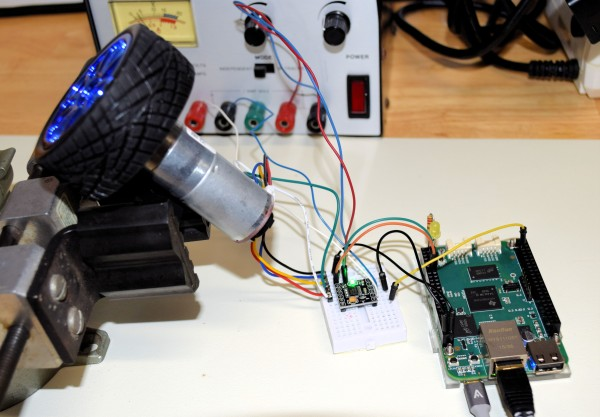
\includegraphics[width=\textwidth]{photos/intro_view}
\end{figure}

\bigskip
{\centering\bfseries\Large
Gregory Raven
\par}


\bigskip
{\centering\bfseries\LARGE
December 28, 2016
\par}
%\newpage





%\setcounter{page}{1}

%\author{Gregory Raven}
%\title{Using the Beaglebone Black Programmable Real-Time Unit with the RemoteProc and Remote Messaging Framework to Capture and Play Data from an ADC}
%\date{October 2016}

%
\frontmatter
Beaglebone Green PRU PID Motor Speed Control Project

Copyright 2016 by Gregory Raven

Some content is based on material published by Texas Instruments.
Please see the TI license agreement included in the Github repository.
%\maketitle
\tableofcontents
\listoftables
\listoffigures
%\maketitle

\mainmatter
%    Documentation for PRU ADC Project
%    Copyright (C) 2016  Gregory Raven
%
%    This program is free software: you can redistribute it and/or modify
%    it under the terms of the GNU General Public License as published by
%    the Free Software Foundation, either version 3 of the License, or
%    (at your option) any later version.
%
%    This program is distributed in the hope that it will be useful,
%    but WITHOUT ANY WARRANTY; without even the implied warranty of
%    MERCHANTABILITY or FITNESS FOR A PARTICULAR PURPOSE.  See the
%    GNU General Public License for more details.
%
%    You should have received a copy of the GNU General Public License
%    along with this program.  If not, see <http://www.gnu.org/licenses/>.

\chapter{Introduction}

This is the documentation for an embedded GNU/Linux project utilizing the RemoteProc and RPMsg framework in the Beaglebone Green (BBG) development board.  The project repository is located here:

\url{https://github.com/Greg-R/pru-pid-motor}

The inspiration for this project came from an example project published by Texas Instruments.  The Texas Instruments project is based on "Code Composer Studio", which is an "Integrated Development Environment" (IDE):

\url{http://processors.wiki.ti.com/index.php/PRU_Training:_PRU_PID_Motor_Demo}

There is also a PDF file which describes the project in detail:

\url{http://www.ti.com/lit/ug/tidubj6/tidubj6.pdf}

The TI project requires a relatively complex cross-compiler installation.  This project is designed to be done via SSH terminal connection, and all software compilation was done on the Beaglebone Green target device using the PRU C compiler (clpru).  The VIM text editor was used to edit files, however, any text editor available in the Debian distribution can be used.

The Debian-based GNU/Linux distribution used on the BBG can be downloaded from this page:

\url{http://beagleboard.org/latest-images}

The ``IOT'' (non-GUI) image was chosen, as this provides the shortest path to get the project up and running.

Recent developments in the Texas Instruments PRU support include the RemoteProc and Remote Messaging frameworks, as well as an extensively documented C compiler and much additional supporting documentation.  This project utilizes these frameworks and is entirely dependent upon C code in both the PRU and GNU/Linux user space.  For further information, refer to the detailed examples provided by TI in the ``PRU Support Package'':

\url{https://git.ti.com/pru-software-support-package}

A listing of additional resources is found in the Resources chapter.

The motor recommended by TI was purchased and tested.  However, a better motor with an integrated quadrature encoder was found on eBay and is recommended.  A chapter is included which describes this motor-encoder and how to obtain one.

\section{Project Goals}

This project demonstrates an electronic speed control for a DC motor which is implemented with the PRUs included with the Beaglebone Green.  Beyond its usefulness as a demonstration project, it could be used in a robotics project such as a ``mobile robot''.

The basic principle of the speed controller is "Proportional Integral Derivative" (PID) feedback control, which is a common feedback controller used in digital systems.

Here is an excellent reference article on PID controllers:

\url{http://www.wescottdesign.com/articles/pid/pidWithoutAPhd.pdf}

\section{Limitations}

All of the development was done as root user via ssh on the BeagleBone Green.  This is generally not a good practice, however, considering this as an embedded and experimental project it was not considered to be a serious drawback.

No attempt was made to optimize the response of the PID controller.  The default values for the PID controller create a stable loop with the recommended DC motor-encoder.  Optimization will depend on the particular motor-encoder chosen and this task is left to the interested experimenter.



%    Documentation for PRU ADC Project
%    Copyright (C) 2016  Gregory Raven
%
%    This program is free software: you can redistribute it and/or modify
%    it under the terms of the GNU General Public License as published by
%    the Free Software Foundation, either version 3 of the License, or
%    (at your option) any later version.
%
%    This program is distributed in the hope that it will be useful,
%    but WITHOUT ANY WARRANTY; without even the implied warranty of
%    MERCHANTABILITY or FITNESS FOR A PARTICULAR PURPOSE.  See the
%    GNU General Public License for more details.
%
%    You should have received a copy of the GNU General Public License
%    along with this program.  If not, see <http://www.gnu.org/licenses/>.

\chapter{System Diagrams}

\begin{figure}[H]
	\centering
	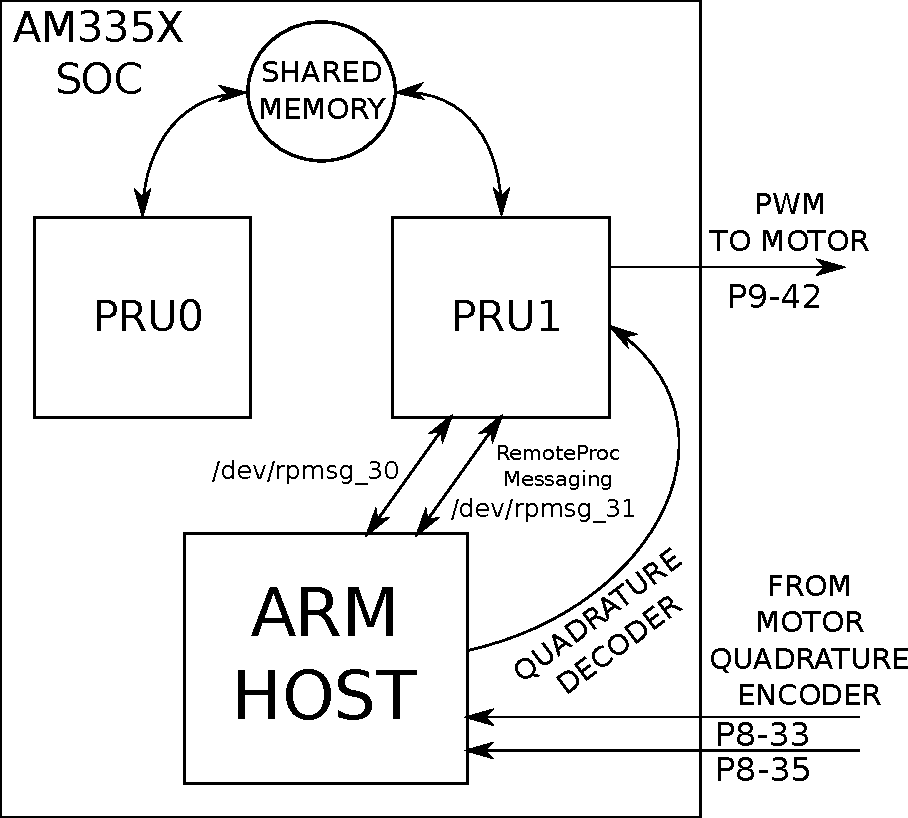
\includegraphics[width=0.8\textwidth]{diagrams/soc_system}
	\centering\bfseries
	\caption{PRU PID System on BeagleBone Green AM335X ``System On Chip''}
\end{figure}

The above diagram shows the data pathways used in the project.  This diagram is a highly simplified view of the AM335X SOC.  Refer to the massively detailed ``Technical Reference Manual'' by Texas Instruments for more information on the internal structure of the AM335X SOC.

\section{Programmable Real-time Units (PRU)}

The system uses both PRUs available on the Beaglebone Green:

\begin{enumerate}
\item 

PRU0 implements the PID controller.  The C code in file PRU\_PID\_0.c contains
the math required for the PID controller.  The controlled quantity is the DC motor RPM which is sensed by the Quadrature Encoder.

PRU0 performs calculations based on data retrieved (and written to) PRU shared memory.
\item 
PRU1 acts as the master controller for the system.  PRU1 instantiates two "character devices" via the RemoteProc Messaging framework.  These character devices are used for two-way communication between the PRUs and Linux user-space.  The PWM module on PRU1 is used to drive the DC motor driver IC.

The Quadrature Encoder used is not contained in the PRU-ICSS.  However, the PRUs have access to the encoders which are part of the AM335X "System On Chip" (SOC) via the OCP Master.  Access to this encoder is enabled in PRU1 code.
\end{enumerate}

It is worth noting that the PRUs each have a copy of the same ``PWMSS'' (Pulse-Width Modulation Subsystem) as the ones located outside the PRU-ICSS in the AM335X SOC.  However, only a single pin is connected from the PRU-ICSS PWMSS to the outside world.  Since this single pin is used for PWM, the decoder-counter function must be done outside the PRU-ICSS. Thus one of the SOC's eQEP decoder-counters is used and is accessed by PRU1 via the OCP Master port.

The PWMSS sub-system is surprisingly complex.  A detailed description of the features of this sub-system is available in the AM335x Technical Reference Manual:

\url{http://www.ti.com/lit/ug/spruh73o/spruh73o.pdf}

\section{PRU Shared Memory}

The firmwares running on the two PRUs use a C structure which is placed into "shared memory".  The shared memory is a part of the PRU-ICSS architecture.  The shared memory is allocated by an entry in the "linker command file" which is included in the Github repository (AM335X\_PRU.cmd).

The structure in shared memory allows the two PRUs to synchronize the PID control parameters.  PRU1 receives these parameters via user-space character devices and then writes them to shared memory.  This makes the parameters available to PRU0, which is then able to perform PID control loop calculations.  PRU0 calculates the PWM duty cycle, and this is written to shared memory.  PRU1 accesses the result and applies this to the PWM output (a duty cycle).

PRU1 is responsible for reading the Quadrature Encoder, which is accessed via the OCP bus master.  PRU1 writes this data to shared memory, which enables PRU0 to access this information for PID loop calculations.

A mystery is how the PRUs are able to share memory without locking.  It is possible for the PRUs to simultaneously read and write to the same memory location without introducing errors?

\section{GNU/Linux Operating System on Host ARM Processor}

The command uname -a on the BBG used to develop this project reports this:

\begin{verbatim}
Linux BBG2 4.4.30-ti-r64 #1 SMP Fri Nov 4 21:23:33 UTC 2016 armv7l GNU/Linux
\end{verbatim}

The latest IOT image has a newer kernel.  It is not a major update as of December 18, 2016.

\section{Motor System Hardware Diagram}

\begin{figure}[H]
	\centering
	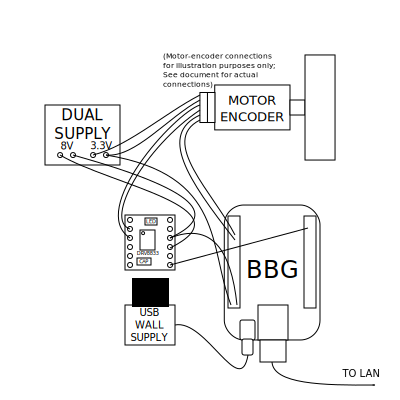
\includegraphics[width=0.8\textwidth]{diagrams/motor_system}
	\centering\bfseries
	\caption{Motor System Hardware Diagram}
\end{figure}

The system was put together as a ``breadboard''.  The DRV8833 carrier board accepts standard header pins, and it easily plugs into a small breadboard.

A bench dual-power supply was used to supply the approximately 8 Volts for the motor.  The second output of the dual supply is set to 3.3 Volts and is connected to the motor-encoder bias supply input.  This supply voltage was found to be somewhat critical and should be adjusted with an oscilloscope to monitor the encoder outputs.

\begin{figure}[H]
	\centering
	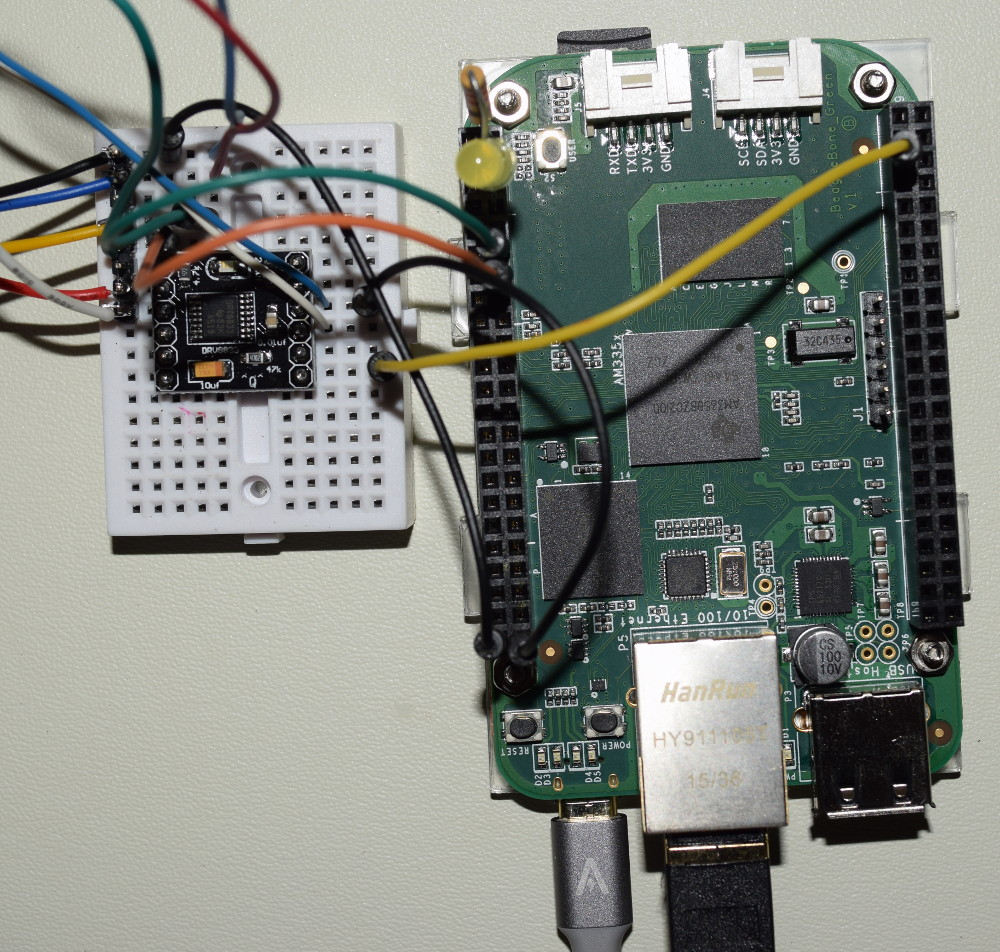
\includegraphics[width=1.0\textwidth]{photos/top_view.jpg}
	\centering\bfseries
	\caption{Photo of the Beaglebone Green and DRV8833 Break-out Boards.  Note the LED/Resistor in series from P8-39 to P8-45.}
\end{figure}






%    Documentation for PRU ADC Project
%    Copyright (C) 2016  Gregory Raven
%
%    This program is free software: you can redistribute it and/or modify
%    it under the terms of the GNU General Public License as published by
%    the Free Software Foundation, either version 3 of the License, or
%    (at your option) any later version.
%
%    This program is distributed in the hope that it will be useful,
%    but WITHOUT ANY WARRANTY; without even the implied warranty of
%    MERCHANTABILITY or FITNESS FOR A PARTICULAR PURPOSE.  See the
%    GNU General Public License for more details.
%
%    You should have received a copy of the GNU General Public License
%    along with this program.  If not, see <http://www.gnu.org/licenses/>.

\chapter{Motor-Encoder}

The TI project recommends using this motor-encoder:

\url{https://www.sparkfun.com/products/13260}

While this motor-encoder kit can be made to work, a better solution was found on eBay:

\begin{figure}[h]
	\centering
    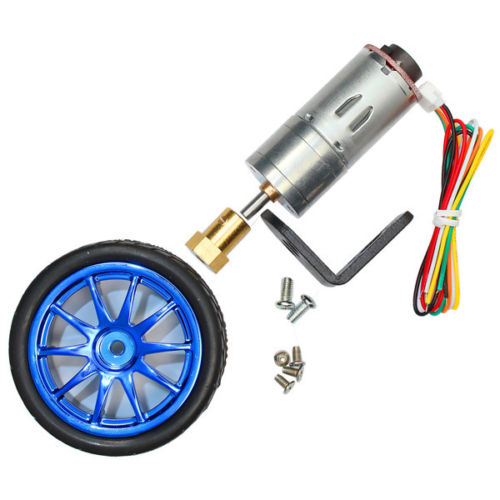
\includegraphics[width=0.5\textwidth]{photos/s-l500.jpg}
	\centering\bfseries
	\caption{eBay Motor-encoder}
\end{figure}

The eBay motor-encoder is a nicely constructed geared DC motor and it has an integrated electronic Quadrature Encoder using Hall-Effect devices.

Also includes is a sturdy mounting bracket, a wired connector, and a brass bushing with matching wheel.  For the purposes of using this in a mobile robot this is very good indeed!

The seller of this motor-encoder was ``kanzezol'' as of December 2016.  This seller also has what appears to be a variant motor-encoder which is less expensive, but it does not include the mounting hardware and wheel.

\section{Quadrature Encoder}

\begin{figure}[h]
	\centering
    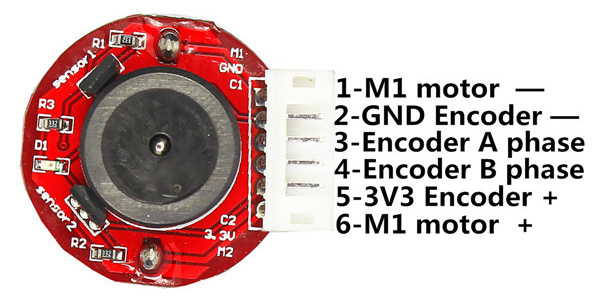
\includegraphics[width=0.5\textwidth]{photos/encoder-close-view.jpg}
	\centering\bfseries
	\caption{The Integrated Quadrature Encoder}
\end{figure}

The suggested DC motor includes an integrated "Quadrature Encoder".  The Quadrature Encoder consists of two Hall-Effect sensors and a rotating magnet attached to the motor shaft.  The rotating magnet has areas of alternating north and south poles.  Thus as the motor shaft turns, the Hall-Effect sensors output a series of pulses with frequency proportional to the rotation velocity "Revolutions Per Minute" (RPM).

Since there are two Hall-Effect sensors, there are two separate pulse outputs.  The Sensors are arranged in physical locations around the rotating magnet such that the two pulse trains overlap.  They overlap with a phase difference of approximately 90 degrees, thus the term "quadrature" is used, however, in practice a precise 90 degree offset does not appear to be critical.

The overlapping pulses allow the sensing of rotational direction, since one sensor will fire first in one direction, and the other sensor will fire first in the opposite direction.  Direction reversal was not included in this project and the feature was not used.

The encoder requires a 3.3 Volt power source.

The 3.3 Volt bias source for the encoder was found to be somewhat critical.  This bias supply could probably be sourced from the BBG, however, this was not attempted.

%    Documentation for PRU ADC Project
%    Copyright (C) 2016  Gregory Raven
%
%    This program is free software: you can redistribute it and/or modify
%    it under the terms of the GNU General Public License as published by
%    the Free Software Foundation, either version 3 of the License, or
%    (at your option) any later version.
%
%    This program is distributed in the hope that it will be useful,
%    but WITHOUT ANY WARRANTY; without even the implied warranty of
%    MERCHANTABILITY or FITNESS FOR A PARTICULAR PURPOSE.  See the
%    GNU General Public License for more details.
%
%    You should have received a copy of the GNU General Public License
%    along with this program.  If not, see <http://www.gnu.org/licenses/>.

\chapter{Motor-Driver Break-out Board DRV8833}

\begin{figure}[h]
	\centering
    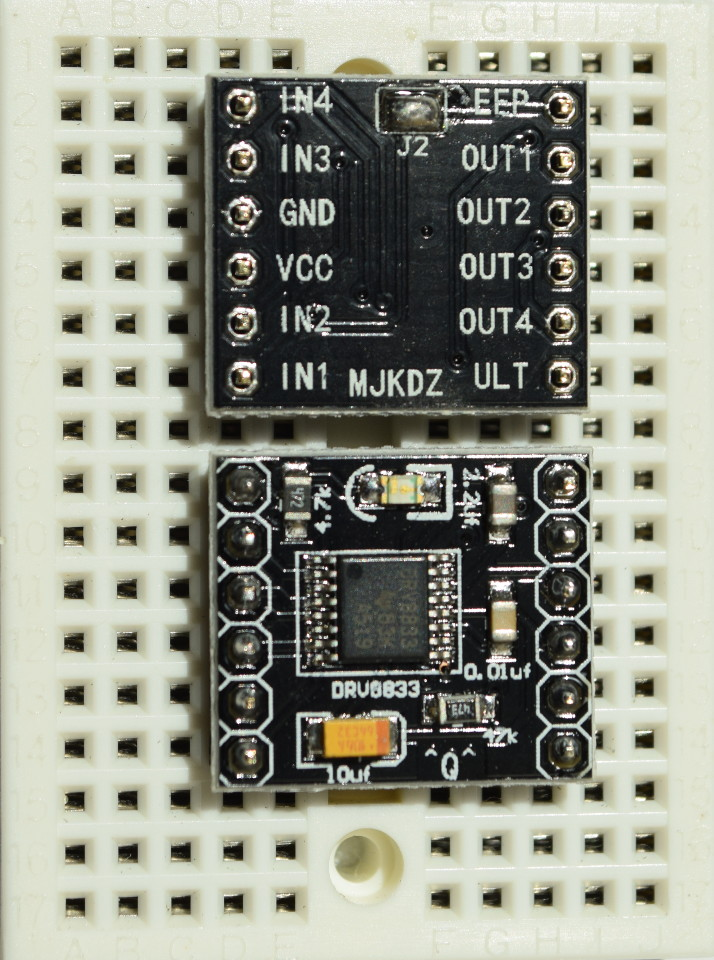
\includegraphics[width=0.5\textwidth]{photos/drv8833_breakout.jpg}
	\centering\bfseries
	\caption{DRV8833 Break-out board (2 boards showing with view of top and bottom sides)}
\end{figure}


The recommended motor driver IC is the Texas Instruments DRV8833:

\url{http://www.ti.com/lit/ds/symlink/drv8833.pdf}

This devices works perfectly with this project and is inexpensive.
Several eBay sellers offer a ``break-out board'' with the IC and several external components mounted with break-board friendly header pin holes.  The board shown in the photo above even includes a surface mounted LED power indicator!

The connections to the board are as follows:

\begin{enumerate}
\item ULT PIN:mode set. Low level is sleep mode
\item OUT1,OUT2:1-channel H-bridge controlled by IN1/IN2
\item OUT3,OUT4:2-channel H-bridge controlled by IN3/IN4
\item EEP PIN:Output protection. Default no need to connect.
\item VCC:3-10V
\item GND
\end{enumerate}

From the above list, only 2, 5 and 6 are used in this project.

IN1 is connected to the PWM output of the BBG, which is header P9.42.
The GND pin requires a connection to one of the grounds on the BBG such as P8.1 or P8.2.

VCC should be connected to an 8Volt DC power supply, however, the exact voltage is not critical.  A solid ground connection should be made between the 8Volt supply and the DRV8833 board.

OUT1 and OUT2 should be connected to the motor power terminals.


\include{./TeX_files/quadrature-decoder.tex}
%    Documentation for PRU ADC Project
%    Copyright (C) 2016  Gregory Raven
%
%    This program is free software: you can redistribute it and/or modify
%    it under the terms of the GNU General Public License as published by
%    the Free Software Foundation, either version 3 of the License, or
%    (at your option) any later version.
%
%    This program is distributed in the hope that it will be useful,
%    but WITHOUT ANY WARRANTY; without even the implied warranty of
%    MERCHANTABILITY or FITNESS FOR A PARTICULAR PURPOSE.  See the
%    GNU General Public License for more details.
%
%    You should have received a copy of the GNU General Public License
%    along with this program.  If not, see <http://www.gnu.org/licenses/>.

\chapter{PRU Firmware and User-space Program}

The ``PRU Firmware'' are two binary files which are placed in the directory /lib/firmware.
These files must have specific names as follows:

\begin{itemize}
	\item am335x-pru0-fw
	\item am335x-pru1-fw
\end{itemize}

The Makefile includes cp commands to copy the firmwares to the /lib/firmware directory.

\section{PID Firmware in PRU0:  Digital Feedback Loop (PRU\_PID\_0.c)}

This C program defines a struct ``shared\_mem'' which contains another struct ``pid\_data''. This same struct is also defined in the PRU1 code.  It is this common data structure which allows the two PRUs to exchange data.

The following code fragment shows how the PRU shared memory is arranged:

\begin{verbatim}
#pragma DATA_SECTION(share_buff, ".share_buff")
volatile far struct shared_mem share_buff;
\end{verbatim}

In addition to the code in the C files, the ``DATA\_SECTION'' must be defined in the linker command file AM335x\_PRU.cmd:

\begin{verbatim}
	  PAGE 2:
	PRU_SHAREDMEM	: org = 0x00010000 len = 0x00002FA8 CREGISTER=28 /* 12kB Shared RAM */
        GLB_BUF         : org = 0x00012FA8 len = 0x00000058 /* Shared buf in Shared RAM */
\end{verbatim}

This must also appear in ``SECTIONS'':

\begin{verbatim}
SECTIONS {
        (...other memory allocations)
        .share_buff > GLB_BUF, PAGE 2
}
\end{verbatim}

The implementation of the PID controller is done using the usual infinite while loop.

A function ``init\_pid'' sets the shared\_mem struct to some initial values.  Another while loop looks for the init\_flag variable to go high, which is a signal from PRU1 that the system is initialized and ready to start.

The main PID control loop is based on the function ``update\_pid''.  The function reads current values from the shared\_mem struct and calculates an error value.  Using the PID controller design pattern, errors for proportional, integral, and derivatives terms are defined in terms of C assignment statements.  The terms are summed to create a total error variable ``output\_f''.

The code uses a ``trick'' to emulate floating point mathematics using only fixed integers:

\begin{verbatim}
output = output_f >> SHIFT;
\end{verbatim}

where the ``SHIFT'' was defined as:

\begin{verbatim}
#define SHIFT    0x0E
\end{verbatim}

The above trick is also applied in the integral statement.

A couple of if statements bound the output within limits set in the shared\_mem struct.

The loop control statement implements the negative feedback control:

\begin{verbatim}
pid->output = pid->max_output - output;
\end{verbatim}

\section{The Firmware in PRU1: PID Control (PRU\_IO\_1.c)}

The firmware in PRU1 is less concerned about math, and more concerned with communicating with the world outside the PRU-ICSS.  The C code sets up the RemoteProc messaging framework to allow communications with Linux user-space.  PRU1 is also responsible for writing to the PWM and reading data from the Quadrature Decoder.

The same shared\_mem struct as seen in PRU0 code is defined.  PRU1 needs to both read and write from this data structure.  PRU0 processes the data and returns an output value to write to the PWM which is determined by the PID calculations.

After initialization, the code enters an infinite while loop.  The while loop services three tasks:

\begin{enumerate}
\item
A RemoteProc Messaging interrupt bit is polled, and if it has been set this means that a message has been sent from Linux user-space.  The message is received, and then an ``interrupt service routine'' function is executed.  The ISR consists mainly of a case statement with several character strings used as codes to either set or read variables in the shared\_mem struct.  This is the mechanism whereby the user-space program can control the motor RPM (setpoint) and parameters of the PID control loop.

\item Write the current output value to the PWM:

\begin{verbatim}
CT_ECAP.CAP2_bit.CAP2 = share_buff.pid.output;
\end{verbatim}

This statement is totally cryptic, but it does indeed write a variable to the PWM function of PRU1 and sets the waveform duty-cycle which in applied to the input of the DRV8833 motor control IC.
\item
Read the Quadrature Decoder output.  This is done using the utility function ``get\_enc\_rpm()''.  Since this is the controlled parameter of the feedback control loop, the value is written to the shared\_mem struct for processing by the PID calculations in PRU0.
\end{enumerate}

The above is only a high-level description, as the code's features are too numerous to describe every function.  The curious reader is invited to examine the code which is published to the Git repository for further details.

\section{Quadrature Decoder Tuning}

The ``Quadrature Decoder'' function is contained within the PWMSS module.  This is a complex system with many tunable parameters.

The original TI project recommends using an LED to signal ``overflow/underflow'' indication from the decoder.  This proved to be important.  The published values for the decoder parameters do not work with the recommended eBay motor-encoder.

The LED indicator is connected to header pin P8-39.  The LED is connected in series with a 1.2k$\Omega$ resistor.  The ground end of the resistor is connected to P8-45.

Universal IO was used to connect the PRU to header pin P8-39 as follows:

\begin{verbatim}
config-pin P8.39 pruout
\end{verbatim}

The above command is included in the shell script ``pru\_gpio\_config''.

Under/over-flow is indicated by a blinking LED which is implemented in the function get\_enc\_rpm().

The following original and modified values are from the function init\_eqep().

\subsection{Original Quadrature Decoder/Encoder Parameters}

This is the original setting for use with the TI recommended motor-encoder; this did not work well with the eBay motor-encoder.  The LED was blinking quite a lot indicating under/overflow in the decoder circuit.

\begin{verbatim}
PWMSS1.EQEP_QCAPCTL = 0x0073;
\end{verbatim}

Another parameter which must be adjusted is the "ticks per revolution".  Due to using a different motor-encoder, and the fact that the motor is geared, this parameter must be changed if the RPM calculation is to be done correctly.  Here is the original parameter:

\begin{verbatim}
/* Encoder definitions */
#define TICKS_PER_REV       16
\end{verbatim}

\subsection{Modified Quadrature Decoder/Encoder Parameters}
    
This value was empirically adjusted until the LED stopped blinking.
The rotation of the motor was ``noisy'' prior to this being adjusted.
With this new value, the motor control changed to smooth and steady.
    
\begin{verbatim}
PWMSS1.EQEP_QCAPCTL = 0x0070;
\end{verbatim}

The parameter for "ticks per revolution" with the eBay motor-encoder is an early estimate:

\begin{verbatim}
/* Encoder definitions */
#define TICKS_PER_REV       40
\end{verbatim}

The above is an early estimate, and it should be re-examined and revised if necessary.  Since this parameter effects the loop dynamics, and the PID parameters had been adjusted for a stable loop, this parameter was left as-is for future optimization.


%    Documentation for PRU ADC Project
%    Copyright (C) 2016  Gregory Raven
%
%    This program is free software: you can redistribute it and/or modify
%    it under the terms of the GNU General Public License as published by
%    the Free Software Foundation, either version 3 of the License, or
%    (at your option) any later version.
%
%    This program is distributed in the hope that it will be useful,
%    but WITHOUT ANY WARRANTY; without even the implied warranty of
%    MERCHANTABILITY or FITNESS FOR A PARTICULAR PURPOSE.  See the
%    GNU General Public License for more details.
%
%    You should have received a copy of the GNU General Public License
%    along with this program.  If not, see <http://www.gnu.org/licenses/>.

\chapter{Shell Scripts}

\section{RemoteProc ``Bind'' and ``Unbind'' Commands}

There are two very important shell scripts located in the shell\_scripts of the git repository.

These scripts are very simple and each contain only a single command.

The commands are described in the notes file from this github repository:

\url{https://github.com/ZeekHuge/BeagleScope}

And specifically, this is the path to the notes file:

\url{https://github.com/ZeekHuge/BeagleScope/blob/port_to_4.4.12-ti-r31%2B/docs/current_remoteproc_drivers.notes} 
	
	The commands are seen in section 2:
	
	\begin{verbatim}
	echo "4a334000.pru0" > /sys/bus/platform/drivers/pru-rproc/unbind
	echo "4a334000.pru0" > /sys/bus/platform/drivers/pru-rproc/bind
	echo "4a338000.pru1"  > /sys/bus/platform/drivers/pru-rproc/unbind
	echo "4a338000.pru1" > /sys/bus/platform/drivers/pru-rproc/bin
	\end{verbatim}
	
	The above shell commands show how the PRUs can ``bind'' and ``unbind'' from the remoteproc driver.  These commands are extremely useful and their placement in shell scripts allows them to be easily run at the command line by entering ``prumodin'' or ''prumodout''.
	
	The shell scripts should be copied to /usr/bin to make them available from any shell.
	
\section{Environment Variables and Universal IO Configuration Script}

The make process which compiles the PRU firmwares requires an environment variable to be set:

\begin{verbatim}
export PRU_CGT=/usr/share/ti/cgt-pru
\end{verbatim}

This is best done by writing this export statement plus other configurations to a file.
This file is sourced from the .bashrc file upon entering the home directory bash shell.

Other methods of setting the environment variables were tried. Using the .bashrc file was found to be the most practical.

When using the ``sudo'' command to gain temporary root access, it is necessary to use the -E option in order to preserve the environment variables.  For example:

\begin{verbatim}
sudo -E make
\end{verbatim}

will preserve the \$PRU\_CGT environment variable and will allow the successful compilation of the PRU firmwares.

The file ``pru\_gpio\_config'' is included in the shell\_scripts directory.  Source the file by adding this line to the end of the .bashrc file located in the user home directory:

\begin{verbatim}
source /home/debian/pru-pid-motor/software/shell_scripts/pru_gpio_config
\end{verbatim}

The path shown above assumes the project was cloned to the user's home directory (debian by default in the latest distribution).

%    Documentation for PRU ADC Project
%    Copyright (C) 2016  Gregory Raven
%
%    This program is free software: you can redistribute it and/or modify
%    it under the terms of the GNU General Public License as published by
%    the Free Software Foundation, either version 3 of the License, or
%    (at your option) any later version.
%
%    This program is distributed in the hope that it will be useful,
%    but WITHOUT ANY WARRANTY; without even the implied warranty of
%    MERCHANTABILITY or FITNESS FOR A PARTICULAR PURPOSE.  See the
%    GNU General Public License for more details.
%
%    You should have received a copy of the GNU General Public License
%    along with this program.  If not, see <http://www.gnu.org/licenses/>.

\chapter{RemoteProc and RPMsg Framework}

\begin{figure}[h]
	\centering
    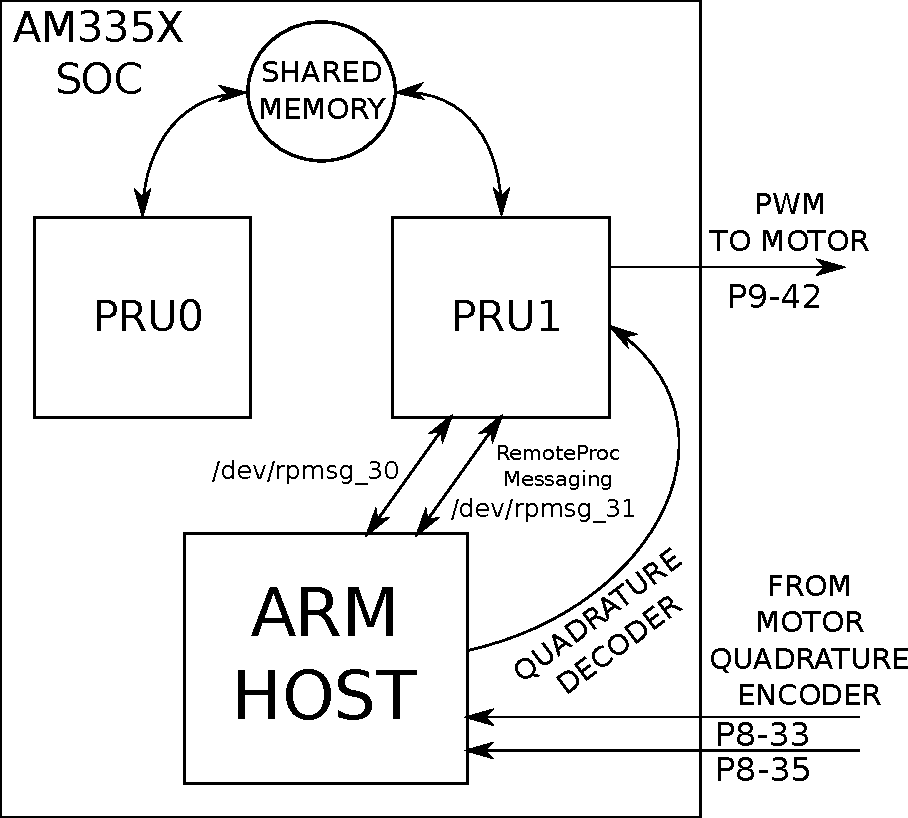
\includegraphics[width=0.7\textwidth]{diagrams/soc_system}
	\centering\bfseries
	\caption{Data Pathways on the AM335X SOC}
\end{figure}

TI has provided example code and kernel drivers for the ``RemoteProc and RemoteProc Messaging Framework''.  A detailed explanation of this framework is available here:

\url{http://processors.wiki.ti.com/index.php/PRU-ICSS_Remoteproc_and_RPMsg}

This framework provides a means of controlling and communicating with the PRUs from user-space, and this project is totally dependent on these functions.

The Remoteproc framework automatically does the job of loading the PRU firmwares from user-space into the PRUs.  Via a sysfs entry, the PRUs can be started and halted from the command line.  These functions are described in the chapter "Shell Scripts".

The examples provided in the PRU Software Support Package show how to use provided functions to send and receive data from PRU to ARM or ARM to PRU.  This is done via character devices which appear in the usual /dev directory.  The standard POSIX functions read/write/open/close work with these character devices.  This allows for typical systems programming technique to be applied when working with the PRUs.

This project uses two character devices assigned to PRU1.  These character devices are used to assign and read back PID parameters to the control system via the user-space executable prumsg.

This project did not require modifications to the loadable kernel modules in the RemoteProc framework.  The modules provided with the IOT Debian-based distribution were used as-is.

\section{The Remoteproc and RPMsg Kernel Modules}

``Loadable Kernel Modules'' (LKMs) must be active for this project to function.
At the shell command line, execute this command:

\begin{verbatim}
lsmod
\end{verbatim}

This will list the LKMs currently loaded.  The modules associated with Remoteproc are:

\begin{itemize}
\item pruss
\item pru\_rproc
\item pruss\_intc
\end{itemize}

There are two modules associated with RPMsg, and these will appear in the list only after the firmwares are loaded into the PRUs:

\begin{verbatim}
virtio_rpmsg_bus
rpmsg_pru
\end{verbatim}

The Remoteproc kernel modules may not be loaded at boot (depending on boot configuration).  However, they can be loaded (or unloaded) anytime after boot with the following commands:

\begin{verbatim}
modprobe pru_rproc
rmmod pru_rproc
\end{verbatim}

``modprobe'' is the load command; ``rmmod'' is the remove command.

Perhaps a better method of controlling the Remoteproc framework is via the sys virtual file system.  A set of shell scripts is included in the repository which includes these commands in the ``prumodout'' and ``prumodin'' scripts.

\section{Files Associated with RemoteProc in the Compilation Process}

There are some interesting files in the root directory of the github repository for this project:

\begin{itemize}
\item resource\_table\_0.h
\item resource\_table\_1.h
\item AM335x\_PRU.cmd
\end{itemize}

These files were copied verbatim from the PRU Support Package.

Jason Reeder of Texas Instruments has provided an explanation of the files required to compile firmwares for the PRUs:

\begin{quotation}
There are four files needed in order to build a C project for the PRU using TI's C compiler. Each of the examples and labs in the pru-software-support-package include these files:
\begin{enumerate}

\item  yourProgramFile.c

This is your C program that you are writing for the PRU.

\item   AM335x\_PRU.cmd

This is a command linker file. This is the way that we describe the physical memory map, the constant table entries, and the placement of our code and data sections (into the physical memory described at the top of the file) to the PRU linker. There are some neat things that can be done as far as placing code and data in exact memory locations using this file, but for the majority of projects, this file can remain unchanged.

\item   resource\_table\_*.h

This file will create a header in the elf binary (generated .out file) that is needed by the RemoteProc Linux driver while loading the code into the PRUs. For the examples in the pru-software-support-package, there are two types of resources that the PRU can request using the resource\_table\_*.h file:

interrupts - letting RemoteProc configure the PRU INTC interrupts saves code space on the PRUs.

vrings - requesting vrings in the resource\_table file is necessary if rpmsg communication is desired (since the ARM/Linux needs to create the vrings in DDR and then notify the PRU where the vrings were placed)
even if no resources are needed, the RemoteProc Linux driver expects the header to exist. Because of this, many examples in the package contain an empty resource\_table header file (resource\_table\_empty.h)

\item   Makefile

Makefile to build your PRU C program either on the target, on your Linux machine, or even on a Windows machine. The comment at the top of the Makefile tries to explain the environment variable needed for a successful build and how to set it on each of the three supported build development environments.  (Note that this is in reference to the Makefiles provided with the PRU Support Package.  The custom Makefile provided with this project does not have this feature.)

\end{enumerate}
\end{quotation}








%    Documentation for PRU ADC Project
%    Copyright (C) 2016  Gregory Raven
%
%    This program is free software: you can redistribute it and/or modify
%    it under the terms of the GNU General Public License as published by
%    the Free Software Foundation, either version 3 of the License, or
%    (at your option) any later version.
%
%    This program is distributed in the hope that it will be useful,
%    but WITHOUT ANY WARRANTY; without even the implied warranty of
%    MERCHANTABILITY or FITNESS FOR A PARTICULAR PURPOSE.  See the
%    GNU General Public License for more details.
%
%    You should have received a copy of the GNU General Public License
%    along with this program.  If not, see <http://www.gnu.org/licenses/>.

\chapter{Device Tree Requirements}

This project requires a custom ``Device Tree Include''.  This is a device tree fragment which is inserted into the top device tree file.  The dtsi directory located in the software directory contains the file and and a README file which explains how to edit the device tree source file.

The same file, which in this case is ``am335x-bonegreen.dts'', must be modified in order to active the RemoteProc framework kernel drivers.  It is recommended to add the include statement at the same time the RemoteProc is activated.  This step is included in the RemoteProc and PRU Compiler step-by-step process in Chapter 9.

There is one PRU GPIO output enabled on header P9 and this is used to monitor Quadrature Decoder under/overflow.  This configuration is done in the same file ``pru\_gpio\_config'' which is sourced by .bashrc as discussed in Chapter 6.

The Universal IO project is located at this Github repository:

\url{https://github.com/cdsteinkuehler/beaglebone-universal-io}

Universal IO is included with the most recent Debian-based IOT images.





%    Documentation for PRU ADC Project
%    Copyright (C) 2016  Gregory Raven
%
%    This program is free software: you can redistribute it and/or modify
%    it under the terms of the GNU General Public License as published by
%    the Free Software Foundation, either version 3 of the License, or
%    (at your option) any later version.
%
%    This program is distributed in the hope that it will be useful,
%    but WITHOUT ANY WARRANTY; without even the implied warranty of
%    MERCHANTABILITY or FITNESS FOR A PARTICULAR PURPOSE.  See the
%    GNU General Public License for more details.
%
%    You should have received a copy of the GNU General Public License
%    along with this program.  If not, see <http://www.gnu.org/licenses/>.

\chapter{Setting up the Remoteproc Framework and PRU Compiler on the Beaglebone Green}

The following describes the simplest possible set-up.  Everything was done via the command line, and the vim editor was used extensively to develop the C code and shell scripts.

SSH was used to remotely access the BBG from a 64 bit desktop computer running Ubuntu 16.04.

For reference, here is the link to the TI PRU support package:

\url{https://git.ti.com/pru-software-support-package}

The above package can be cloned to the BBG.  There is a good set of examples and labs included.  The labs are documented here:

\url{http://processors.wiki.ti.com/index.php/PRU_Training:_Hands-on_Labs}

Note that the files appropriate for the BBG are in the folders with name am335x.

The Makefiles in the labs and examples were designed to work with a particular set-up which can be easily implemented on the BBG.

The following is a list of recommended steps to prepare a BBG for compiling PRU C files.
This process assumes a recent SD card image (IOT recommended) which is loaded with the PRU compiler (clpru) and libraries.  Another assumption is that the RemoteProc and RPMsg kernel drivers are included and that they are loaded during the start-up process.  This is true for some, but not all, recently published images as of December, 2016.

\section{Activate RemoteProc PRU and Kernel Modules}

The newest Beaglebone Debian distributions do not have the Remoteproc framework activated by default!

The following process activates the framework which includes several loadable kernel modules.  This is a prerequisite for the remainder of the setup process.

This process was tested using this image:

bone-debian-8.6-iot-armhf-2016-10-30-4gb.img

The ``IOT'' (Internet Of Things) image includes the set of tools required to install and compile the required software.
The image was found at this web site:

\url{http://elinux.org/Beagleboard:BeagleBoneBlack_Debian#microSD.2FStandalone:_.28iot.29_.28BeagleBone.2FBeagleBone_Black.2FBeagleBone_Green.29}

The IOT distribution includes very useful scripts in the following directory:

/opt/scripts/tools

The script grow\_partition.sh will expand the file system on the micro-sd card to its full capacity.  Running this script is highly recommended before proceeding with this process!

\section{Activate Remoteproc: Step-by-step Process}

\begin{enumerate}
\item  Write Beaglebone image to micro-sd and expand partition as required.
\item  Insert micro-sd into BBG slot, press boot and power buttons and release.  Non-flasher images may not require the boot button to be pressed, and the board will boot and run from the micro-sd card automatically.
\item  ssh debian@192.168.1.7 (or whatever the IP is set to).  If you are using a router with a GUI control application, it may have a display which indicates the board is connected and to which IP address has been assigned to it.
\item  Execute
\begin{verbatim}
sudo apt-get update
\end{verbatim}
\item  Execute
\begin{verbatim}
uname -r
\end{verbatim} 
to verify kernel version.  Please note that the RemoteProc framework is still evolving and it is recommended to verify that the kernel used will work with the PRU support package examples.

The rest of the set-up will be completed using root access.
Execute
\begin{verbatim}
sudo su
\end{verbatim}
and authenticate if required to switch to root user.
\item Clone this repository to a convenient directory (recommended /opt/scripts/tools):

\begin{verbatim}
git clone https://github.com/RobertCNelson/dtb-rebuilder
\end{verbatim}

\item Execute:
\begin{verbatim}
cd dtb-rebuilder/ 
cd src/arm
\end{verbatim}
\item Find and edit the top of the device tree dts file.
For BBG, this is:
\begin{verbatim}
am335x-bonegreen.dts
\end{verbatim}
Uncomment this single line in the file:
\begin{verbatim}
/*   #include "am33xx-pruss-rproc.dtsi"  */
\end{verbatim}

The line should now look like this:
\begin{verbatim}
#include "am33xx-pruss-rproc.dtsi"
\end{verbatim}

A new include statement must be added to the same file for configuration of the Quadrature Decoder and the PRU PWM.  This file must be copied from the repository:

\begin{verbatim}
pru-pid-motor/software/dtsi/am335x-boneblack-prupid.dtsi
\end{verbatim}

into the arm directory in the dtb-rebuilder.

Add this line to the end of the am335x-bonegreen.dts file:

\begin{verbatim}
#include "am335x-boneblack-prupid.dtsi"
\end{verbatim}
 
Save and exit.
\item
Execute:
\begin{verbatim}
cd /etc/modprobe.d
\end{verbatim}
Create a new file named:
\begin{verbatim}
pruss-blacklist.conf
\end{verbatim}
Note that the latest images may already have this file.

Add this single line to the file:
\begin{verbatim}
blacklist uio_pruss
\end{verbatim}
Save and exit.
\item
cd back to the dtb-rebuilder directory.  Execute these commands:
\begin{verbatim}
make 
make install 
reboot
\end{verbatim} 
\end{enumerate}
To verify that the above process was successful:

\begin{verbatim}
cd /sys/bus/platform/devices
ls
\end{verbatim}

Now look for the following in the output from the ls command:
\begin{verbatim}
4a300000.pruss
4a320000.intc
4a334000.pru0
4a338000.pru1
\end{verbatim}

The appearance of the above entries indicates that the RemoteProc PRU activation process was successful.

\section{PRU Compiler Setup Process}

\begin{enumerate}
\item  Execute these commands:
\begin{verbatim}
cd /
\end{verbatim} and then 
\begin{verbatim}
find . -name cgt-pru
\end{verbatim}

The path should be something like 
\begin{verbatim}
/usr/share/ti/cgt-pru
\end{verbatim}  

This is the location of the PRU library and includes.
However, the clpru compiler binary is not located in this directory.  Run this command:
\begin{verbatim}
which clpru
\end{verbatim}
and the result will be something like:
\begin{verbatim}
/usr/bin/clpru
\end{verbatim}
This is the path to the compiler binary.

The PRU C compiler needs to find the include and lib directories.  The Makefiles in the PRU Support Package look for the compiler binary at this path, so the following changes must be made.

Execute the following commands (as root):
\begin{verbatim}
cd /usr/share/ti/cgt-pru
mkdir bin
cd bin
ln -s /usr/bin/clpru clpru
\end{verbatim}
So now the Makefiles will find the compiler executable in the correct location via the link.
\item  Now install the PRU Support Package in the home directory:

\begin{verbatim}
cd /home/debian
git clone git://git.ti.com/pru-software-support-package/pru-software-support-package.git
\end{verbatim}

This will clone a copy of the latest pru support package.
\item  cd into lab\_5 in the package and execute the make command:
\begin{verbatim}
cd pru-software-support-package/labs/lab_5/solution/PRU_Halt
make
\end{verbatim}
This will fail, as the Makefile is looking for environment variable \$PRU\_CGT.  Execute:

\begin{verbatim}
export PRU_CGT=/usr/share/ti/cgt-pru
\end{verbatim}

Now execute the make command again.  It should succeed.  A new directory ``gen'' should appear.  The above command is included in the file ``pru\_gpio\_config'' in the shell\_scripts directory of the project's Github repository.

\item  Execute the following:
\begin{verbatim}
cd gen
cp PRU_Halt.out am335x-pru0-fw
cp am335x-pru0-fw /lib/firmware
\end{verbatim}
This renames the executable binary and copies it to the directory at which Remoteproc expects to find PRU firmwares.
\item  Now cd into the PRU\_RPMsg\_Echo\_Interrupt1 directory in the same lab\_5.
Edit main.c as follows:
\begin{verbatim}
//#define CHAN_NAME					"rpmsg-client-sample"
#define CHAN_NAME					"rpmsg-pru"
\end{verbatim}
The ``CHAN\_NAME'' define is now set to ``rpmsg-pru''.
\item  Now execute almost the same as \#9, except this time the firmware for PRU1 is compiled a copied:
\begin{verbatim}
make
cd gen
cp PRU_RPMsg_Echo_Interrupt1.out am335x-pru1-fw
cp am335x-pru1-fw /lib/firmware
\end{verbatim}
The compilation of both PRU firmwares are complete and they are copied to /lib/firmware.
\item  reboot
\item  Execute:

\begin{verbatim}
lsmod
\end{verbatim}

These kernel modules should be present in the output:

\begin{verbatim}
pru_rproc              15431  0 
pruss_intc              8603  1 pru_rproc
pruss                  12026  1 pru_rproc
\end{verbatim}
Now execute:
\begin{verbatim}
rmmod pru_rproc
modprobe pru_rproc
\end{verbatim}

The rmmod command removes the remoteproc module pru\_rproc.
The modprobe command re-inserts the same module.
\item  
\begin{verbatim}
cd /dev
ls
\end{verbatim} 

Look for rpmsg\_pru31 character device file.  It will be there!
This confirms that the PRU C compiler are properly configured and that the Makefile for this project will compile the PRU binaries successfully.  The RemoteProc drivers are also tested with the successful completion of the above set-up process.  This is not the entire configuration, however.
\end{enumerate}

\section{Additional Configuration Required to Compile the PRU Remoteproc Project}

Some components of the PRU Support Package need to be added to the PRU C compiler directories.  The Makefile expects to find these components in these directories.

Execute these commands in the directory in which the PRU Support Package was cloned:

\begin{verbatim}
cd pru-software-support-package/
cp -r include $PRU_CGT/includeSupportPackage
cp lib/rpmsg_lib.lib $PRU_CGT/lib
\end{verbatim}

This should complete the configuration required to run the project's Makefile successfully.




%    Documentation for PRU ADC Project
%    Copyright (C) 2016  Gregory Raven
%
%    This program is free software: you can redistribute it and/or modify
%    it under the terms of the GNU General Public License as published by
%    the Free Software Foundation, either version 3 of the License, or
%    (at your option) any later version.
%
%    This program is distributed in the hope that it will be useful,
%    but WITHOUT ANY WARRANTY; without even the implied warranty of
%    MERCHANTABILITY or FITNESS FOR A PARTICULAR PURPOSE.  See the
%    GNU General Public License for more details.
%
%    You should have received a copy of the GNU General Public License
%    along with this program.  If not, see <http://www.gnu.org/licenses/>.

\chapter{Running the Project}

It is assumed the numerous steps described in prior chapters have been completed to enable the RemoteProc framework drivers and configure the BBG for compiling PRU C code.  The Device Tree must have been successfully edited and re-compiled and installed, and the shell scripts prumodin and prumodout have been copied to /usr/bin.

In order to run the project and successfully control the motor, follow these steps:

\begin{itemize}
	\item run ``make'' in the software repository directory.  Some warnings or errors may be ignored.  Check that the C code files prumsg.c, PRU\_PID\_0.c and PRU\_IO\_1.c compile and firmware files am335x-pru0-fw and am335x-pru1-fw are copied to /lib/firmware.  The user-space binary prumsg should be copied to /usr/bin.
	
	\item Run command 
	
	\begin{verbatim}
	prumodin
	\end{verbatim} 
	
	at the command line.  This command should start firmware execution in the PRUs.
	If all goes well, the motor should begin turning with a default setpoint value of 3000.
	
	\item  Finally, the user-space program can be used.
	
	\begin{verbatim}
	sudo ./prumsg s 4000
	\end{verbatim}
	
	The above command changes the setpoint to 4000 rpm.  The motor speed should increase.
\end{itemize}

The PRU firmwares will continue to run.  To stop them, issue the commands

\begin{verbatim}
sudo prumodout
sudo rmmod pru_rproc
sudo rmmod pruss
\end{verbatim}

at the command line, and the PRUs will be halted.  The motor will stop.

\section{User-space Program prumsg Command Listing}

The user-space executable file prumsg is capable of several control and monitoring functions.  These commands are issued from a shell and a complete listing of the possible commands is listed below.

\begin{longtable}{ll}
\caption{Commands of User-space Program prumsg}\\
\toprule
Example command & Command function \\\midrule
prumsg 30 s 5000 & Set setpoint (RPM) \\ 
prumsg 30 p 300 & Set Kp, proportional feedback coefficient \\ 
prumsg 30 i 300 & Set Ki, integral feedback coefficient \\ 
prumsg 30 d 300 & Set Kd, derivative feedback coefficient \\ 
prumsg 30 o 3000 & Set output PWM duty cycle (see note below) \\ 
prumsg 30 rs & Readback setpoint (RPM) \\ 
prumsg 30 rp & Readback Kp \\ 
prumsg 30 ri & Readback Ki \\ 
prumsg 30 rd & Readback Kd \\ 
prumsg 30 re & Readback encoder RPM \\
prumsg 30 ro & Readback output PWM
\end{longtable}

Notes on the above:
\begin{enumerate}
\item If not operating as root, ``sudo'' will be required.
 
\item ``30'' in the table above refers to the character device /dev/rpmsg\_pru30.  ``31'' can also be used, as this character device is also established between PRU1 and user-space.
 
\item The example for setting the PWM (prumsg 30 o 3000) will not have effect with the PID controller running.  However, this command is useful for debugging purposes.  If the PID controller is not running in PRU0, then the command will work and the PWM output will change.  The simplest way to do this is to remove firmware am335x-pru0-fw from directory /lib/firmware.  Reboot and restart the system.  PRU1 will still function in system control mode, but the PID calculations will not be performend by PRU0 and the system will operate in ``open-loop'' mode.  This is excellent for checking the PWM output to the motor driver IC and the motor connections.  The motor should properly respond to changes in the PWM duty cycle by issuing the prumsg 30 s (pwm value) command.
\end{enumerate}

\section{Server and GUI Interface from TI Project}

The TI project includes a very clever PHP web page and server interface.  This was found to be mostly functional, and the server shell script and web page implementation is included in the pru\_pid\_server directory of the Git repository.

The server is easy to run.  Simply copy the contents of the pru\_pid\_server directory to /var/www/html which should already be included in the Beaglebone Green IOT image.

Now, using a browser on the local network, browse to this URL:

\begin{verbatim}
10.0.0.2:8080
\end{verbatim}

In the above example, the BBG is set to a static IP of 10.0.0.2.

This was found to partially function, the graphics successfully updates, however, the capability to update the setpoint and PID parameters did not function.

This project does not support this function.  Since the Beagleboard project is heavily invested in node.js and ``Bonescript'', it would probably make sense to change this function from PHP/html to a node-based web interface and use a web-socket for data exchange and parameter control.  This feature may be added in the future to this project.

%    Documentation for PRU ADC Project
%    Copyright (C) 2016  Gregory Raven
%
%    This program is free software: you can redistribute it and/or modify
%    it under the terms of the GNU General Public License as published by
%    the Free Software Foundation, either version 3 of the License, or
%    (at your option) any later version.
%
%    This program is distributed in the hope that it will be useful,
%    but WITHOUT ANY WARRANTY; without even the implied warranty of
%    MERCHANTABILITY or FITNESS FOR A PARTICULAR PURPOSE.  See the
%    GNU General Public License for more details.
%
%    You should have received a copy of the GNU General Public License
%    along with this program.  If not, see <http://www.gnu.org/licenses/>.

\chapter{Resources}

\section{Github repository for this project}

\url{https://github.com/Greg-R/pru-pid-motor}

\section{The Texas Instruments PRU PID Motor Demonstration Project}


\url{http://processors.wiki.ti.com/index.php/PRU_Training:_PRU_PID_Motor_Demo}

There is also a PDF file which describes the project in detail:

\url{http://www.ti.com/lit/ug/tidubj6/tidubj6.pdf}

\section{Texas Instruments PRU Code Generation tools}

\url{http://software-dl.ti.com/codegen/non-esd/downloads/download.htm#PRU}

\section{Beagle Bone Green}

\url{https://www.seeedstudio.com/SeeedStudio-BeagleBone-Green-p-2504.html}

\section{The Remoteproc Framework and Remote Messaging}

\url{http://processors.wiki.ti.com/index.php/PRU-ICSS_Remoteproc_and_RPMsg}

\section{The PRU GPIO Spreadsheet}

Use ``git clone'' to download this repository:

\url{https://github.com/selsinork/beaglebone-black-pinmux}

The spreadsheet file contained in this repository is pinmux.ods.
The LibreOffice suite has a spreadsheet application which will read
this file.

This spreadsheet is extremely useful when configuring the PRU or
other functions to the Beaglebone pin multiplexer.

\section{The BeagleScope project}

``Beaglescope'' includes some very important information on the RemoteProc framework:

\url{https://github.com/ZeekHuge/BeagleScope}


\backmatter
% bibliography, glossary and index would go here.

\end{document}
